\documentclass[sigconf,nonacm]{acmart}

\usepackage{graphicx}
\usepackage{xcolor}
\usepackage{listings}
\usepackage{float}
\usepackage{algorithm}
\usepackage{algpseudocode}
\usepackage{amsmath}

% C++ code listing style
\lstdefinestyle{cppstyle}{
    language=C++,
    basicstyle=\ttfamily\small,
    keywordstyle=\color{blue}\bfseries,
    commentstyle=\color{gray},
    stringstyle=\color{magenta},
    numbers=left,
    numberstyle=\tiny,
    stepnumber=1,
    showstringspaces=false,
    tabsize=2,
    breaklines=true,
    frame=single,
    captionpos=b
}
\lstset{style=cppstyle}

\title{DH2323 Project Report}
\subtitle{\url{https://github.com/Maximilian-Benedicto/DH2323-project}}

\date{15 May 2026}

\author{Maximilian Benedicto \\ 20031103-5216}
\email{mbene@kth.se}
\affiliation{%
    \institution{KTH Royal Institute of Technology}
    \city{Stockholm}
    \country{Sweden}}

\author{Arman Montazeri \\ DITT PERSONNUMMER HÄR}
\email{armanmo@kth.se}
\affiliation{%
    \institution{KTH Royal Institute of Technology}
    \city{Stockholm}
    \country{Sweden}}

\renewcommand{\shortauthors}{Benedicto and Montazeri}

\begin{document}

\begin{teaserfigure}
    \centering
    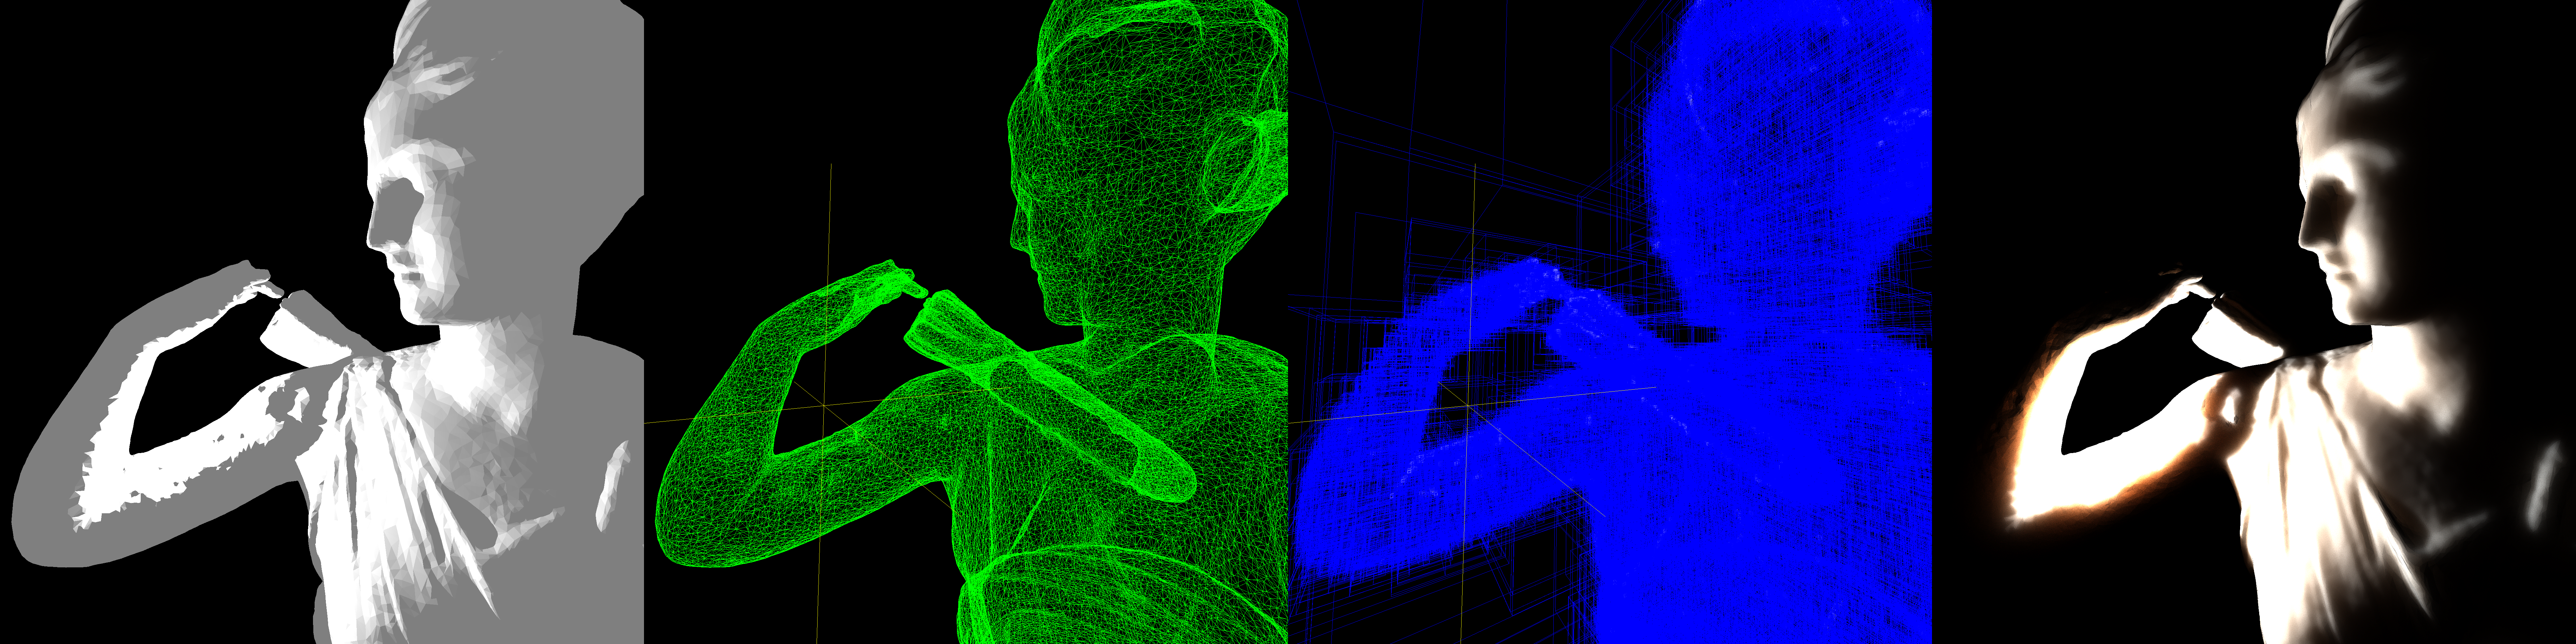
\includegraphics[width=\textwidth]{../img/DianaGrid1000Samples.png}
    \caption{Marble statue rendered with Lambertian, Wireframe, BVH, and Dipole shaders.}
    \Description{A grid of images illustrating a marble statue rendered using Lambertian, Wireframe, BVH, and Dipole shaders.}
    \label{fig:teaser}
\end{teaserfigure}

\begin{abstract}
    In this report, we present an implementation of subsurface scattering using a BSSRDF model based on the dipole approximation by Jensen et al. We developed a modular C++ rendering framework that supports complex geometries and interactive navigation through multithreaded, tile-based rendering. The system aims to simulate the characteristic translucent "glow" of materials like marble and milk by decoupling light transport into single and multiple scattering components. While the implementation successfully produces soft shadows, we observe certain visual discrepancies compared to the original study. We discuss these results in relation to our simplified lighting model and outline future strategies for performance and perceptual evaluation.
\end{abstract}

\maketitle

\section{Introduction}

The Bidirectional Reflectance Distribution Function (BRDF) is a fundamental concept widely utilized in computer graphics. It is a five-dimensional function, defined as the ratio of outgoing radiance to incident irradiance, which characterizes how a material reflects light for any given pair of incident and outgoing directions at a specific wavelength \cite{sun2021bidirectional}. In previous coursework, we employed a simplified form of the BRDF, the Lambertian model, which assumes that light reflectance is ideally diffuse and occurs at the exact point of incidence.

While the BRDF is valuable, it fails to account for subsurface scattering, a phenomenon critical for accurately rendering translucent materials such as milk, skin, or marble. Subsurface scattering occurs when light enters an object's surface, scatters internally, and exits from a different location \cite{adobe2026subsurface}. This effect is essential for achieving true photorealism, providing a depth and softness that surface-only lighting models cannot replicate. Subsurface scattering is formally described by the Bidirectional Scattering-Surface Reflectance Distribution Function (BSSRDF). The BRDF is, in fact, a simplified special case of the BSSRDF where the entry and exit points are assumed to be identical.

Jensen et al. \cite{jensen2001practical} introduced a practical BSSRDF model that is significantly more computationally efficient than pre-existing methods, such as the heavy Monte Carlo simulations previously required to solve subsurface scattering problems. Jensen's model achieves its efficiency through a hybrid approach: it combines an exact analytical solution for single scattering with a diffusion-based approximation for multiple scattering.

This model defines the total BSSRDF as the sum of these two distinct components:
\begin{equation}
    S(x_i, \vec{\omega}_i; x_o, \vec{\omega}_o) = S_d(x_i, \vec{\omega}_i; x_o, \vec{\omega}_o) + S^{(1)}(x_i, \vec{\omega}_i; x_o, \vec{\omega}_o).
\end{equation}

The single scattering term, $S^{(1)}$, accounts for light that enters the medium, undergoes exactly one scattering event, and then exits. This is derived from the analytical integration of radiance along the light's path within the volume:
\begin{equation}
    L_o^{(1)}(x_o, \vec{\omega}_o) = \frac{\sigma_s(x_o) F p(\vec{\omega}_i \cdot \vec{\omega}_o)}{\sigma_{tc}} e^{-s'_i \sigma_t(x_i)} e^{-s'_o \sigma_t(x_o)} L_i(x_i, \vec{\omega}_i).
\end{equation}

Conversely, the multiple scattering term approximates light that has scattered numerous times and become isotropic. This is modeled using the dipole approximation, which treats internal light transport as a diffusion process:
\begin{equation}
    S_d(x_i, \vec{\omega}_i; x_o, \vec{\omega}_o) = \frac{1}{\pi} F_t(\eta, \vec{\omega}_i) R_d(\|x_i - x_o\|) F_t(\eta, \vec{\omega}_o).
\end{equation}

\section{Related Work}

This project builds upon the foundational paper ``A Practical Model for Subsurface Light Transport'' by Jensen et al. \cite{jensen2001practical}, as well as the prior project on Subsurface Scattering by Curran \cite{curranmax2013subsurface}, which was itself a direct implementation of Jensen's model.

\section{Methodology}

Our initial focus was on thoroughly analyzing and understanding the theoretical framework presented by Jensen et al. \cite{jensen2001practical}. Because the mathematical formulations appeared complex at first glance, we utilized Gemini Deep Research \cite{google2026gemini} to clarify interconnected formulas and establish a logical starting point for the codebase. Furthermore, we cross-referenced the underlying theory with existing open-source implementations, specifically Curran's work \cite{curranmax2013subsurface}, to bridge the gap between mathematical models and \texttt{C++} code.

Once the theoretical foundation was solidified, we constructed a custom rendering framework. This system was largely inspired by the architectures developed in previous coursework (specifically Labs 2 and 3). We engineered a program capable of loading complex geometries in both \texttt{.obj} and \texttt{.ply} formats, alongside the standard Cornell Box scene. A central architectural goal was to create a modular system that allowed seamless toggling between different rendering algorithms and 3D models. This approach not only reinforced ray tracing fundamentals, such as intersection handling and texture mapping, but also provided a reliable baseline against which we could compare our results after implementing the dipole method.

We began integrating the dipole method by directly translating the core mathematical formulas into code. By implementing these equations to observe their data dependencies prior to fully grasping their roles, we were forced to reason critically about necessary data types and structures. A significant realization during this phase was that material properties vary across the RGB spectrum, necessitating independent calculations for each color channel. By leveraging the GLM library, we treated these spectral properties as vectors, which streamlined the mathematical expressions and allowed parallel processing of all three color channels. Through this iterative coding methodology, we developed a deep intuition for how the various components interacted.

\section{Implementation}

\subsection{Multithreaded Shaders}

The rendering system is organized around three distinct shader classes: Lambertian, Wireframe, and Dipole. The Wireframe and Lambertian shaders were developed using techniques introduced in Labs 2 and 3, providing both a structural visualization of the geometry and a standard diffuse lighting model for baseline comparisons. All shaders integrate seamlessly with the course-provided \texttt{Window} class to handle display output and the user interface.

Given the substantial computational cost of ray tracing, both the Lambertian and Dipole shaders employ a parallelized rendering architecture. We optimized the rendering process by subdividing the screen space into a $4 \times 4$ grid, yielding $16$ independent tiles. Each tile is processed by a separate thread, distributing the CPU workload and drastically reducing the time required to render a full frame.

Maintaining camera responsiveness is a primary challenge in real-time ray tracing; computationally heavy frames can easily cause the application to stall. To mitigate this, we implemented an atomic flag: a signal that forces all active rendering threads to abort their current workload immediately if camera movement is detected. Instead of blocking the thread to finish a stale frame, the system discards the obsolete work and prioritizes the updated view. This interrupt-driven architecture guarantees smooth, lag-free scene navigation, resuming high-quality rendering only when the camera comes to a rest.

\subsection{Bounding Volume Hierarchy (BVH)}

\begin{figure}[H]
    \centering
    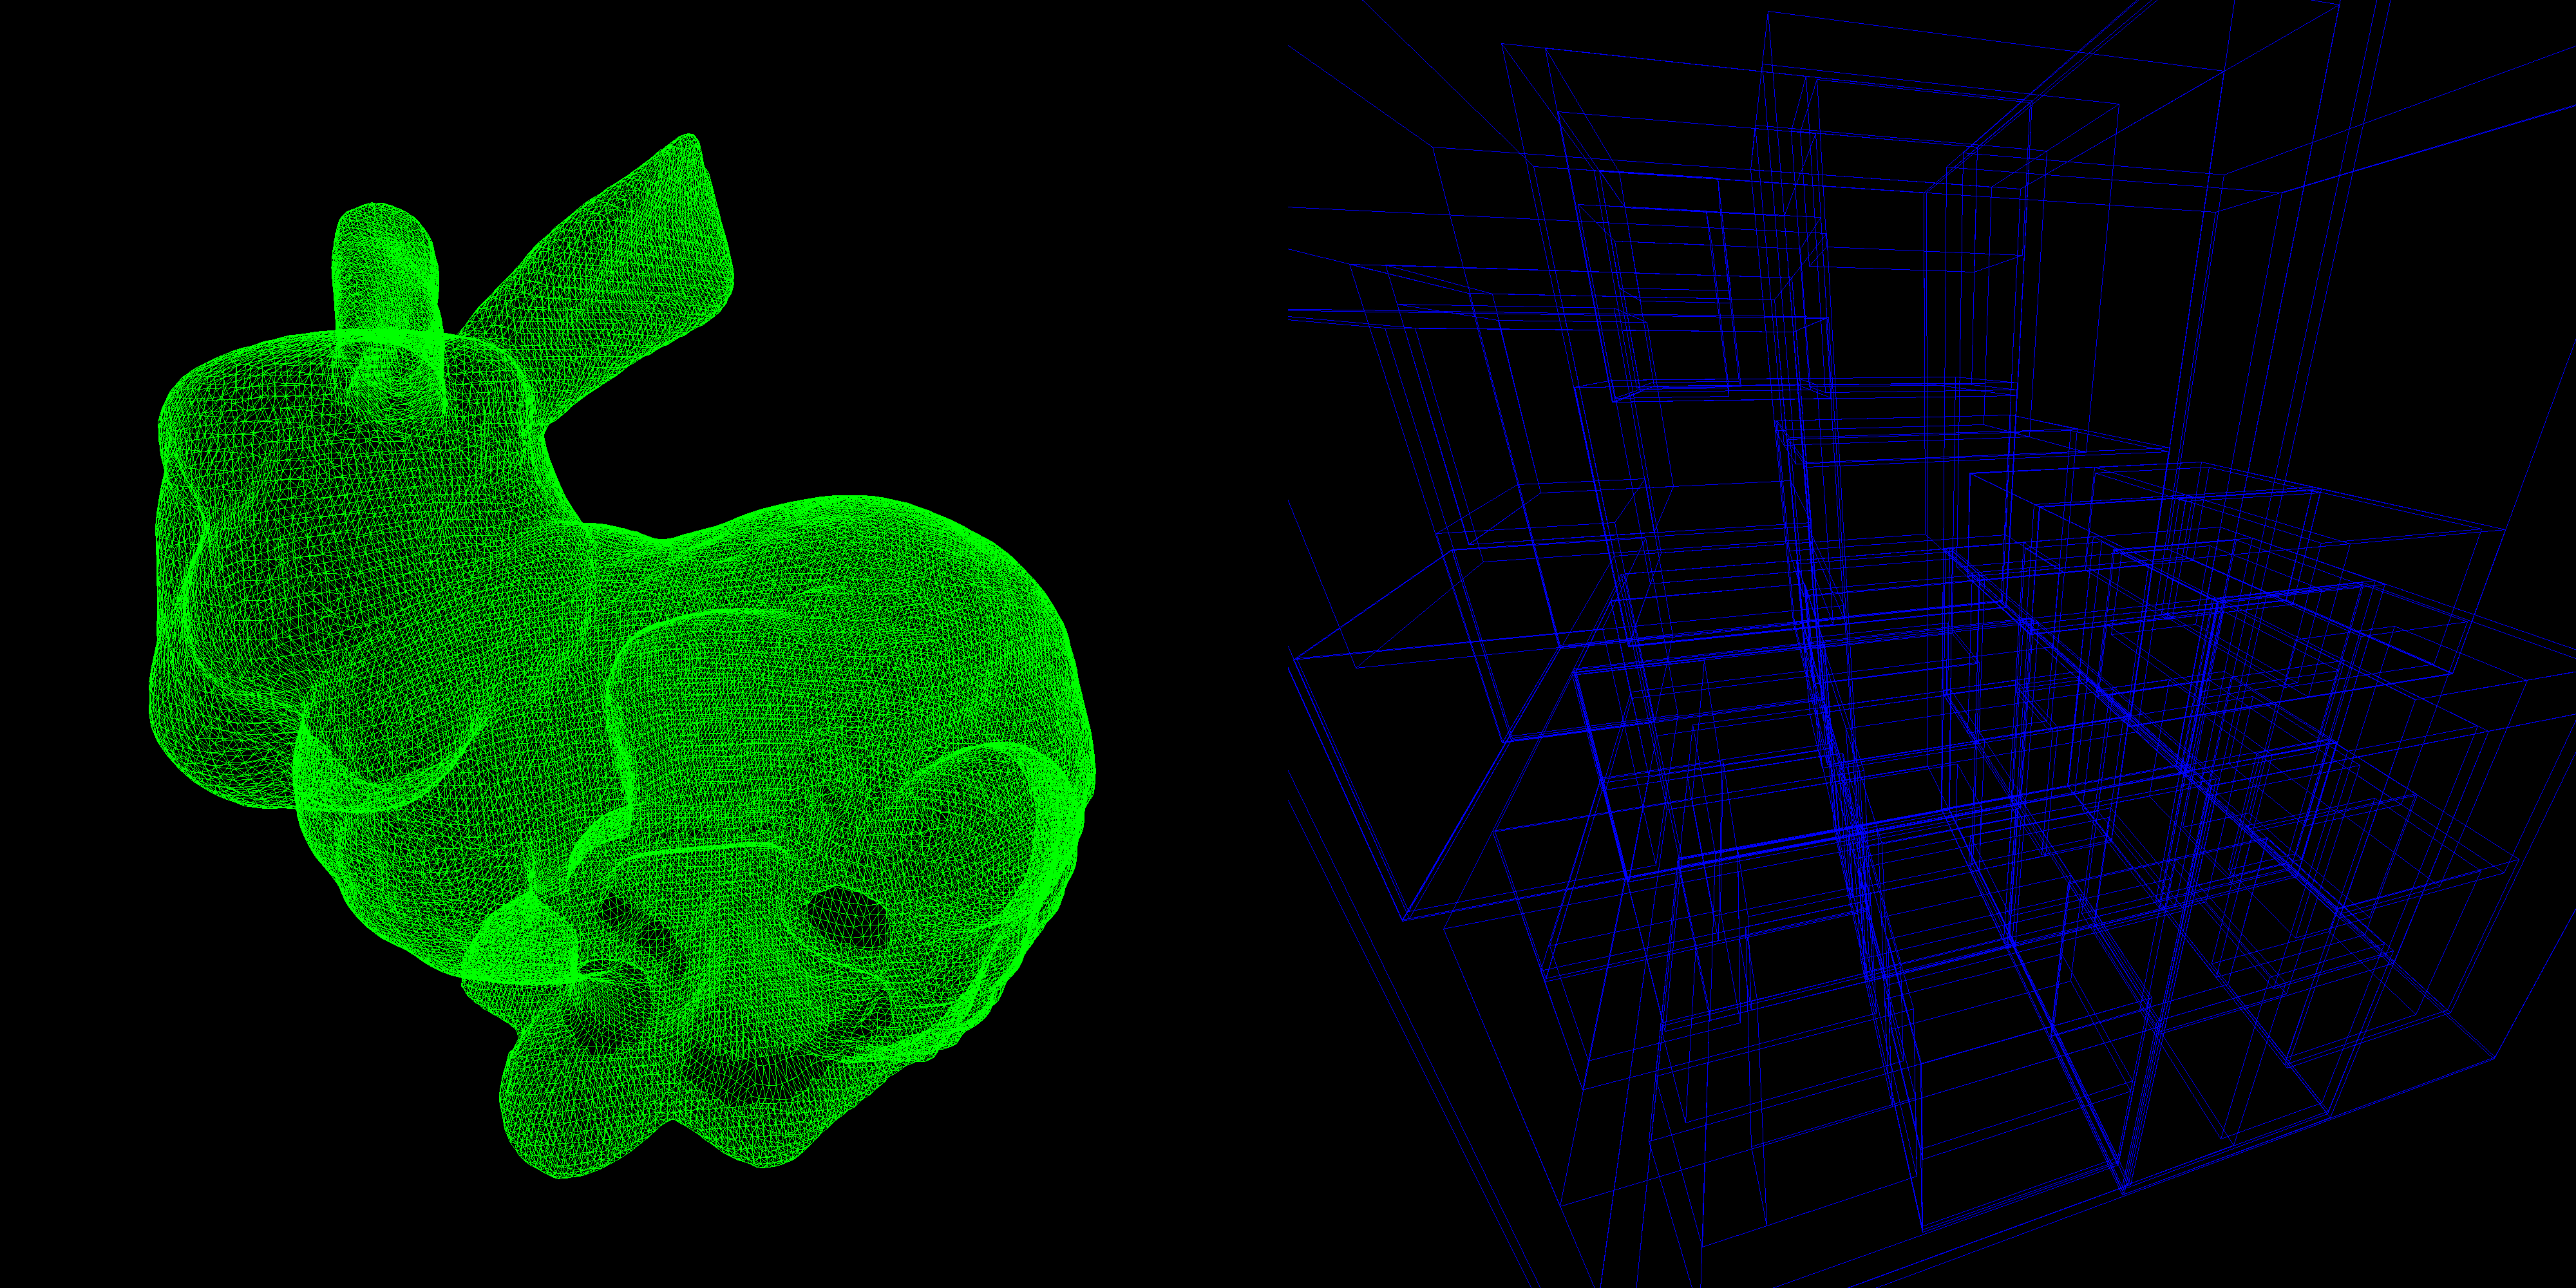
\includegraphics[width=0.45\textwidth]{../img/BunnyGrid1000Triangles.png}
    \Description{Wireframe rendering of the Stanford Bunny alongside a 3D visualization of its recursively subdivided bounding volume hierarchy boxes.}
    \caption{The Stanford Bunny wireframe model and its corresponding bounding volume hierarchy.}
    \label{fig:bunny}
\end{figure}

To accelerate ray-triangle intersection tests, a Bounding Volume Hierarchy (BVH) \cite{pharr2018physically} was implemented. This data structure organizes triangles into a tree hierarchy where leaf nodes contain the actual geometric primitives, and branch nodes store the bounding boxes of all primitives nested beneath them. The tree is constructed recursively by splitting the scene's triangles based on a chosen heuristic, in our case dividing them evenly along the axis with the largest extent. This acceleration structure drastically reduces intersection tests; rather than checking every triangle in the scene, the algorithm only traverses branches whose bounding boxes intersect the ray.

To minimize overhead and pointer complexity, our implementation flattens the entire tree into a one-dimensional \texttt{std::vector}. The root node is stored at index $0$, and the left and right children of any node $i$ are located at indices $2i+1$ and $2i+2$, respectively. Two fundamental data structures form the backbone of this system: \texttt{AABB} and \texttt{BVHNode}.

The Axis-Aligned Bounding Box (\texttt{AABB}) defines a rectangular volume aligned with the $x$-, $y$-, and $z$-axes that encapsulates the underlying geometry. Defined by its minimum and maximum coordinate bounds, the structure includes methods for expanding the box to contain a new point or another \texttt{AABB}.

\begin{lstlisting}[style=cppstyle]
struct AABB {
    glm::vec3 min;
    glm::vec3 max;

    void grow(glm::vec3 p);
    void grow(const AABB& b);
};
\end{lstlisting}

The \texttt{BVHNode} struct represents either a branch or a leaf node. If it operates as a branch node, it contains the index of its left child in the BVH vector and signals its branch status by maintaining a triangle count of zero. If it is a leaf node, it stores both the starting index of its triangles (within the global triangle array) and the number of triangles it contains.

\begin{lstlisting}[style=cppstyle]
struct BVHNode {
    AABB aabb;

    int leftFirst;
    int triCount;

    bool isLeaf() const { return triCount > 0; }
};
\end{lstlisting}

The BVH is constructed using a recursive, top-down methodology:
\begin{enumerate}
    \item Initialize the root node to contain the entire triangle array.
    \item Compute the node's \texttt{AABB} to bound every triangle
    \item If the node contains fewer triangles than the maximum leaf threshold, mark it as a leaf and terminate the branch.
    \item Otherwise, compute the bounding box of the triangle centroids and identify the axis with the largest spatial extent.
    \item Calculate the split position as the midpoint of the centroid bounds along the chosen axis.
    \item Partition the triangles in-place.
    \item If partitioning results in an empty subset, halt further division.
    \item Instantiate left and right child nodes referencing the two sub-ranges, update their respective \texttt{AABB}s, and recursively subdivide them.
\end{enumerate}

Ray intersections with the BVH are executed via an iterative depth-first traversal:
\begin{enumerate}
    \item Initialize an explicit stack with the root node.
    \item Pop the top node and test its \texttt{AABB} against the ray using the slab method \cite{wikipedia2026slab}. If the ray misses, skip the node entirely.
    \item If the node is an internal branch, push its intersecting children onto the stack (prioritizing the nearer child).
    \item If the node is a leaf, evaluate every contained triangle using the Möller--Trumbore \cite{wikipedia2026moller} intersection algorithm, tracking the closest valid hit.
    \item Repeat until the stack is empty. Return the closest intersection found, if any.
\end{enumerate}

Once all relevant leaf nodes have been tested, the traversal terminates, yielding the closest intersection point. For a perfectly balanced tree containing $N$ triangles, the best-case time complexity is $\mathcal{O}(\log N)$, representing a massive performance improvement over the naive $\mathcal{O}(N)$ approach.

\subsection{Material}

\begin{figure}[H]
    \centering
    \includegraphics[width=0.45\textwidth]{../img/CornellGrid1000Samples.png}
    \Description{Grid of 12 Cornell Box scenes, each demonstrating one of the twelve measured translucent materials, such as milk, marble, skin, and apple.}
    \caption{Cornell Box, scaled to 5.55 cm across, rendered with all 12 materials.}
    \label{fig:cornell}
\end{figure}

In addition to formulating the dipole method, Jensen et al. provided real-world empirical measurements for the model's fundamental constants. These values serve the dual purpose of validating the model against physical reality and providing ready-to-use parameters for rendering accurate materials. The primary physical constants are the reduced scattering coefficient ($\sigma_s'$), the absorption coefficient ($\sigma_a$), and the relative index of refraction ($\eta$). The original paper catalogs these constants for 12 distinct materials: Apple, Chicken1, Chicken2, Cream, Ketchup, Marble, Potato, Skimmilk, Skin1, Skin2, Spectralon, and Wholemilk.

In our \texttt{C++} architecture, these fundamental constants and their derived properties are encapsulated within a \texttt{Material} class. This class stores $\sigma_s'$, $\sigma_a$, and $\eta$, and computes the necessary derived coefficients \eqref{eq:material_constants}. The anisotropy constant $g$ (the mean cosine of the scattering angle) is assumed to be $0.85$, adhering to Jensen's specifications.

\begin{subequations}
    \label{eq:material_constants}
    \begin{align}
        F_{dr}      & = -\frac{1.440}{\eta^2} + \frac{0.710}{\eta} + 0.668 + 0.0636 \eta, \\
        \sigma_s    & = \frac{\sigma_s'}{1 - g},                                          \\
        \sigma_t'   & = \sigma_a + \sigma_s',                                             \\
        \alpha'     & = \frac{\sigma_s'}{\sigma_t'},                                      \\
        \sigma_{tr} & = 3 \sigma_a \sigma_t',                                             \\
        A           & = \frac{1 + F_{dr}}{1 - F_{dr}},                                    \\
        D           & = \frac{1}{3 \sigma_t'},                                            \\
        z_r         & = \frac{1}{\sigma_t'},                                              \\
        z_v         & = z_r + 4 A D.
    \end{align}
\end{subequations}


\subsection{Single and Multiple Scattering}

The total radiance exiting a point $x_o$ is determined by summing the independent contributions of single and multiple scattering. Consequently, these elements can be evaluated separately. Each contribution is computed via a two-stage process: sampling followed by radiance evaluation. First, importance sampling selects entry points ($x_i$) on or within the medium. Second, Monte Carlo integration estimates the total radiance contributed by these sampled paths.

\subsubsection{Sampling}

The mathematical core of the sampling logic relies on Monte Carlo importance sampling. This technique generates sample points distributed according to a specific probability density function (PDF) and weights their contributions inversely by that probability. The integral is thereby approximated as a weighted average:

\begin{equation}
    I \approx \frac{1}{N} \sum_{i=1}^{N} \frac{f(x_i)}{p(x_i)}.
\end{equation}

For both single and multiple scattering, the PDF is dictated by the material's optical constants. Because these constants are defined as RGB vectors, we simplify the sampling heuristic by averaging the three color channels to determine the scalar probabilities used for ray generation.

In the single-scattering simulation, the penetration distance $d$ along the refracted outgoing ray is sampled from the exponential density function $\sigma_t e^{-\sigma_t d}$. This determines the internal scatter point $s$, representing the physical location where the photon interacts with the medium. From this scatter point, a shadow ray is traced toward the light source; the intersection of this ray with the geometric boundary defines the incident entry point $x_i$. The distances from $x_i$ to $s$ and from $s$ to $x_o$ are denoted as $s_i$ and $s_o$, respectively, and are used in the radiance evaluation step.

\begin{figure}[H]
    \centering
    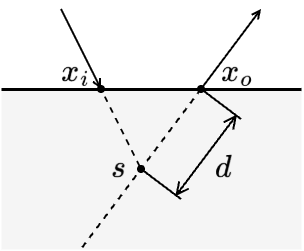
\includegraphics[width=0.2\textwidth]{../img/SingleScattering.png}
    \Description{Diagram defining the geometry of single scattering: an incoming ray enters at the boundary, travels to an internal point, scatters once, and exits.}
    \caption{The scatter point $s$ is sampled at distance $d$ along the refracted ray.}
    \label{fig:single_scattering}
\end{figure}

For the multiple scattering approximation, potential entry points ($x_i$) are sampled across a planar disc situated tangent to the exit point ($x_o$). The radial distance $r$ from $x_o$ is sampled using the density profile $\sigma_{tr} e^{-\sigma_{tr} r}$, while the angle $\theta$ is sampled uniformly between $0$ and $2\pi$. Local tangent and bitangent vectors are computed to establish an orthogonal basis for the tangent plane, which is used to map the polar coordinates $(r, \theta)$ into 3D world space.

\begin{figure}[H]
    \centering
    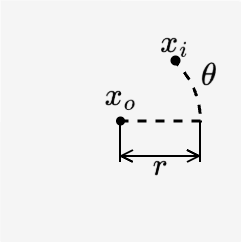
\includegraphics[width=0.2\textwidth]{../img/MultipleScattering.png}
    \Description{Diagram of the multiple scattering approximation, showing a tangent disc situated at the exit point used to sample entry points across its surface.}
    \caption{The entry point $x_i$ is sampled across a tangent disc at $x_o$ using polar coordinates.}
    \label{fig:multiple_scattering}
\end{figure}

\subsubsection{Radiance Calculation}

To accurately evaluate the radiance at the exit point, several helper functions are implemented within the shader. These include Schlick's approximation \cite{wikipedia2026schlick} for the Fresnel reflectance ($F_r$) and transmittance ($F_t$), the dipole diffusion profile ($R_d$), and the Henyey-Greenstein phase function \cite{wikipedia2026henyey} ($p$). The complete set of evaluating equations is defined as follows:

\begin{subequations}
    \label{eq:radiance_calculation}
    \begin{align}
        F_0                                  & = \left( \frac{1 - \eta}{1 + \eta} \right)^2,                                                                                                                    \\
        F_r(\vec{\omega}_i ; \vec{\omega}_o) & = F_0 + (1 - F_0)(1 - (\vec{\omega}_i \cdot \vec{\omega}_o))^5,                                                                                                  \\
        F_t(\vec{\omega}_i ; \vec{\omega}_o) & = 1 - F_r(\vec{\omega}_i \cdot \vec{\omega}_o),                                                                                                                  \\
        d_r                                  & = \sqrt{r^2 + z_r^2},                                                                                                                                            \\
        d_v                                  & = \sqrt{r^2 + z_v^2},                                                                                                                                            \\
        R_d(r)                               & = \frac{\alpha'}{4\pi} \left[ \frac{z_r(\sigma_{tr} d_r + 1) e^{-\sigma_{tr} d_r}}{d_r^3} + \frac{z_v(\sigma_{tr} d_v + 1) e^{-\sigma_{tr} d_v}}{d_v^3} \right], \\
        p(\vec{\omega}_i ; \vec{\omega}_o)   & = \frac{1 - g^2}{4\pi (1 + g^2 - 2g (\vec{\omega}_i \cdot \vec{\omega}_o))^{3/2}}.
    \end{align}
\end{subequations}

With the sample points generated and material parameters deduced, the total single and multiple scattering components are independently calculated via Monte Carlo integration over $N$ samples. To find the incident radiance $L_i$ in our specific lighting model, a shadow ray is cast to test visibility against the single point light source. If unoccluded, $L_i$ is evaluated using an inverse-square distance falloff. The exact algorithms for single and multiple scattering radiances are outlined in \eqref{alg:single_scattering} and \eqref{alg:multiple_scattering}, respectively.

\begin{algorithm}[H]
    \caption{Radiance evaluation for single scattering.}
    \begin{algorithmic}
        \Function{SingleScattering}{$x_o, \vec{\omega}_o$}
        \State $L^{(1)} \gets 0$
        \State Calculate exit Fresnel transmittance $F_{to}$ at $x_o$
        \For{$i = 1$ to $N$}
        \State Sample entry point $x_i$, density $p_i$, and distances $s_i$, $s_o$
        \State Cast shadow ray from $x_i$ to light source
        \If{shadow ray is occluded}
        \State \textbf{continue}
        \EndIf
        \State Calculate incident radiance $L_i$ and direction $\vec{\omega}_i$ at $x_i$
        \State Calculate entry Fresnel transmittance $F_{ti}$ at $x_i$
        \State Evaluate phase function $P \gets p(\vec{\omega}_i \cdot \vec{\omega}_o)$
        \State Calculate transmittances $T_i \gets e^{-\sigma_t s_i}$ and $T_o \gets e^{-\sigma_t s_o}$
        \State $L_{contrib} \gets \sigma_s L_i F_{ti} F_{to} P \, T_i \, T_o$
        \State $L^{(1)} \gets L^{(1)} + \frac{L_{contrib}}{p_i}$
        \EndFor
        \State \Return $\frac{L^{(1)}}{N}$
        \EndFunction
    \end{algorithmic}
    \label{alg:single_scattering}
\end{algorithm}

\begin{algorithm}[H]

    \caption{Radiance evaluation for multiple scattering.}
    \begin{algorithmic}
        \Function{MultipleScattering}{$x_o, \vec{\omega}_o$}
        \State $L_d \gets 0$
        \State Calculate exit Fresnel transmittance $F_{to}$ at $x_o$
        \For{$i = 1$ to $N$}
        \State Sample entry point $x_i$ on tangent disc, density $p_i$
        \State Cast shadow ray from $x_i$ to light source
        \If{shadow ray is occluded}
        \State \textbf{continue}
        \EndIf
        \State Calculate incident radiance $L_i$ and direction $\vec{\omega}_i$ at $x_i$
        \State Calculate entry Fresnel transmittance $F_{ti}$ at $x_i$
        \State Evaluate diffuse reflectance $R_d(\|x_i - x_o\|)$
        \State $L_{contrib} \gets \frac{1}{\pi} (\vec{n}_i \cdot \vec{\omega}_i) L_i F_{ti} R_d F_{to}$
        \State $L_d \gets L_d + \frac{L_{contrib}}{p_i}$
        \EndFor
        \State \Return $\frac{L_d}{N}$
        \EndFunction
    \end{algorithmic}
    \label{alg:multiple_scattering}
\end{algorithm}

\section{Future Perceptual Study}

To formally evaluate the visual efficacy of our implementation, a future perceptual user study should be conducted. The primary objective would be to quantify how closely our dipole-based renders approximate the ground-truth standard established by path-traced Monte Carlo simulations. In this proposed study, participants would be shown rendered images and tasked with identifying the depicted materials (e.g., milk, marble, or ketchup) without prior knowledge of what each entails. By cross-referencing recognition success rates between our model and the Monte Carlo reference, we could empirically gauge the perceptual accuracy of the diffusion approximation.

Furthermore, this study would facilitate an analysis of the model's reliability across varying material classes. Preliminary observations indicate that the dipole approximation excels with highly translucent, low-absorption materials like marble, where light transport is heavily diffusion-dominated. However, for materials with starkly different scattering profiles (e.g., ketchup), the dipole assumptions may yield less accurate visual approximations compared to a brute-force simulation. A structured perceptual study would yield concrete data highlighting exactly which material properties are faithfully captured by Jensen's model and where the diffusion approximation begins to break down.

If this project were to inform a broader, interactive application space, such as a real-time game or interactive simulation, the perceptual study would also need to address trade-offs between physical accuracy and rendering time. For instance, testing an optimization where single scattering is entirely omitted for distance-based objects could reveal how visually discerning the human eye is regarding distant subsurface effects. While the exact mathematical accuracy drops significantly, the resulting performance gain might be vast, with minimal degradation to the human-perceived image. Such findings would bridge the gap between physically-based rendering principles and real-time rendering logic.

\subsection{Evaluation}

Beyond a purely perceptual study, a rigorous mathematical evaluation could be performed to verify the algorithmic correctness of our implementation. Alongside their provided material constants, Jensen et al. included schematics of the laboratory apparatus used to measure these empirical values. We could digitally reconstruct this measurement environment within our framework and compare our software-simulated diffuse reflectance against their physical laboratory readings. This quantitative approach would allow us to definitively assert the physical accuracy of our software.

\section{Conclusion}

Our implementation presents promising results in rendering subsurface scattering effects, though several limitations remain. The marble statue render produced is visually appealing but does not perfectly replicate the reference image, possibly due to incorrect model, scaling, or lighting parameters. This discrepancy highlights differences in implementation that cannot be fully resolved through visual comparison alone. In particular, our analysis revealed a disproportionate contribution from the multiple scattering term relative to single scattering, indicating an imbalance in our lighting and material configuration.

The material Spectralon behaved as expected, exhibiting diffuse surfaces and sharply defined shadows, lending some confidence to the correctness of our model. However, rendering other translucent materials proved more challenging. While soft shadows were achieved, characteristic bright edges around objects were not observed, suggesting limitations in our approach. These differences may arise from our simplified lighting setup, which uses a single point light source and evaluates only direct light reachability scaled by inverse squared distance, rather than integrating incident radiance over the full hemisphere. A more rigorous evaluation could be achieved by replicating the original measurement setup, allowing iterative refinement toward physically accurate results.

Developing this rendering framework involved notable challenges but also deepened our understanding of light transport. While implementing ray-tracing structures such as BVH, intersection logic, and multithreading was straightforward due to ample existing resources, bridging Jensen et al.'s BSSRDF theory with functional \texttt{C++} code required a careful, modular approach. By isolating each equation and verifying its data dependencies, we successfully translated complex optical physics into a structured software architecture, paving the way for future refinements and validation against physical measurements.

\section{Contribution \& Acknowledgements}

Both members collaborated equally on all aspects of the project, including theoretical analysis, code implementation, and report writing. We utilized pair-programming techniques to ensure that both members had a comprehensive understanding of the entire codebase and theoretical framework.

\textbf{Use of AI Tools:} We utilized Gemini Deep Research as a theoretical aid to clarify and break down the mathematical formulations from the original Jensen et al. paper. AI was used strictly as an educational tool to bridge our understanding of the physics and to assist with debugging complex equations. All final \texttt{C++} code, structural design, and report text were authored entirely by the project members.

\bibliographystyle{ACM-Reference-Format}
\bibliography{references}

\end{document}